\section{Results and Discussion}
\label{sec:results}

\subsection{Inferred velocities}

In this section we assess the quality of the 3D stellar velocities we infer.
Figure \ref{fig:results} shows the distribution of stellar velocities inferred
for 5000 randomly selected Kepler stars.
The 2D distributions of inferred stellar velocities are plotted in the
lower-left panels, with black contours indicating the stellar number density.
The red contours in these panels show the marginal projections of the
Gaussian prior in 2D.
The diagonal panels show the 1D distributions (histograms) of stellar
velocities.
The black histogram shows the distribution of inferred velocities, the cyan
histogram shows the distribution of velocities calculated for stars with RVs
(on which the prior was based), and the red lines show the 1D prior
distributions.
The prior distribution was calculated using the velocities of stars with RVs.
If the velocity distributions of stars were Gaussian, the 1D red Gaussians
would look like the cyan histograms.
In other words, the differences between the red lines and cyan histograms
is caused by the non-Gaussianity of the velocity distributions.
This figure is intended to highlight the differences and similarities
between the inferred stellar velocities and the prior distributions.
In each panel, the distribution of inferred velocities is fairly similar to
the distribution of directly-measured velocities; the velocities of stars
calculated with and without RVs are broadly similar.
The inferred \vx\ and \vz\ velocities, and distances are relatively
precise, with median uncertainties of \vxprecision \kms, \vzprecision\ \kms,
and \dprecision\ kpc, respectively.
The inferred \vy\ velocities have a median uncertainty of \vyprecision\ \kms.

% Among stars with measured RVs, \vy\ and \vz\ are slightly positively
% correlated, \ie\ stars with larger \vy\ tend to have larger \vz.
There is a slight negative correlation between inferred \vy\ and \vz\
velocities, which is visible in the central panel of figure \ref{fig:results}.
This negative correlation is not seen in the prior, nor is it apparent in the
posteriors of individual stars: figure \ref{fig:posterior} shows that the \vy\
and \vz\ parameters are {\it positively} correlated for KIC \kicstar.
This negative correlation may be due to the specific orientation of the Kepler
field, which creates a slight degeneracy between \vy\ and \vz.
% , and could
% result in a negative correlation in the population of stars that is not
% apparent in the posteriors of individual stars.
% To an observer looking at Kepler field, a star with either a positive
% \vz\ or a {\it negative} \vy\ would appear to move in the direction of
% positive \vz, when projected onto the sky.
% In this sense, \vy\ and \vz\ are negatively correlated.
% However, the observed proper motions of a star without a measured RV could be
% equally well described by either increasing both \vy\ and \vz, or decreasing
% both \vy\ and \vz.
% For this reason, the star's posterior PDF over \vy\ and \vz\ will be
% positively correlated.
% This could result in a paradoxical result whereby the posteriors over vy and
% vz are positively correlated for individual stars, however the vy and vz
% velocities of the population are negatively correlated.
If this explanation is correct, this phenomenon highlights how apparent
correlations in stellar velocities could result from {\it missing}
information.
This point is interesting, but the effect is relatively small and we do not
expect that this observed correlation between \vz\ and \vy\ will significantly
affect kinematic age studies.

% could have {\it
% either} a positive \vz, or a postitive \vy. with a positive
% \vz\
% This difference is caused by the way the inaccuracies in inferred \vy\
% velocities manifest in the \vz\ velocity distribution.
% Although correlation patterns appear between the inferred velocities as a
% result of marginalizing over RV, the inferred velocities are still consistent
% with their `true' velocities.
% The proper motions of stars with a given \vy\ and \vz\ could be equally
% well-described with a slightly larger \vy\ and a smaller \vz\ or vice versa.

\begin{figure}[ht!]
\caption{
The distribution of inferred stellar velocities and distances.
    Figure \ref{fig:results} shows the inferred velocities of 5000 randomly
selected Kepler stars.
The 2D distributions of inferred stellar velocities are plotted in the
lower-left panels, with black contours indicating the stellar number density.
The red contours in the lower-left panels show the marginal projections of
    the Gaussian prior distribution in 2D.
The upper-right panels in the figure, lying on the plot's diagonal, show the
    1D distributions (histograms) of stellar velocities.
The black histogram shows the distribution of inferred velocities, the blue
histogram shows the distribution of velocities for stars with RVs,
and the red lines show the 1D marginal Gaussian prior distributions.
This figure shows that the distributions of inferred velocities are
    broadly similar to the distributions of velocities directly calculated
    using RVs, and the prior constructed from them.
}
  \centering
    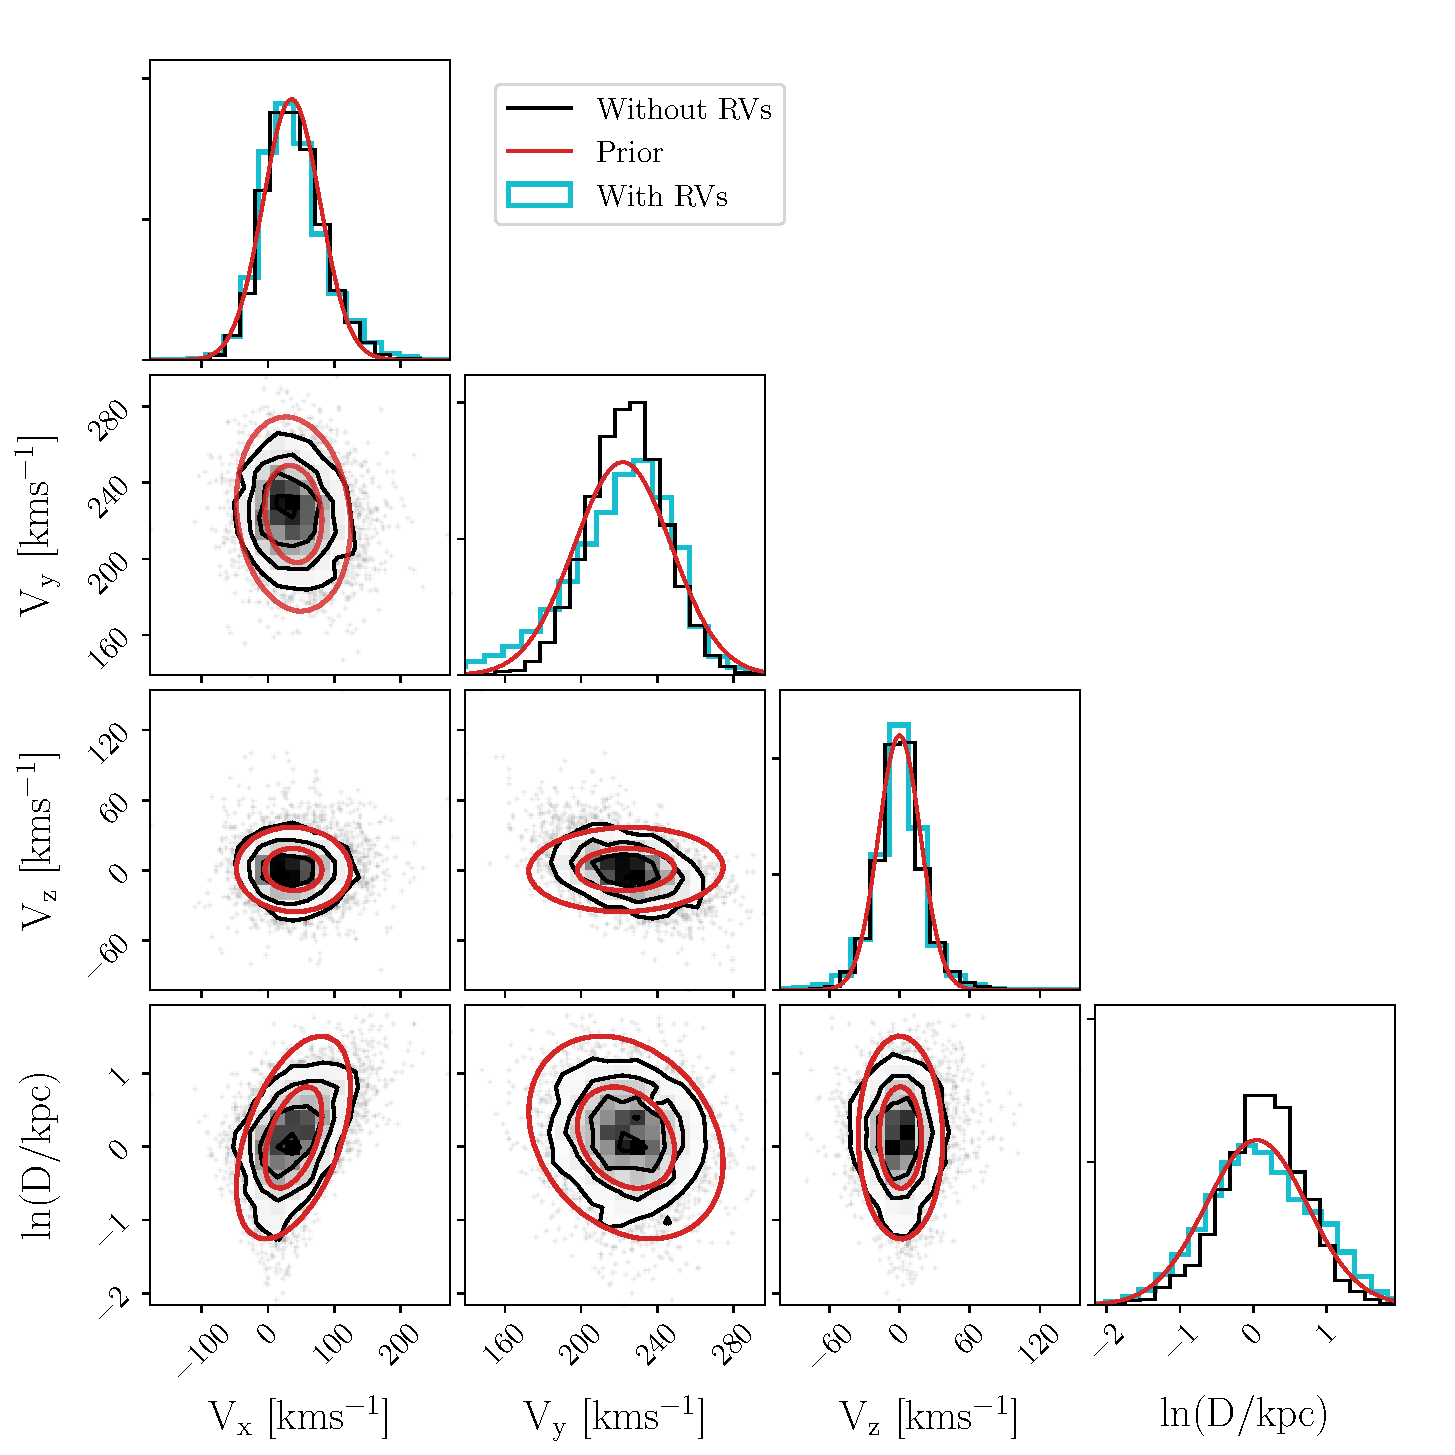
\includegraphics[width=.7\textwidth]{results_figure}
\label{fig:results}
\end{figure}
To further validate our method, we compare inferred velocities with
directly-calculated velocities for stars in our sample with measured RVs.
Figure \ref{fig:residuals} shows the \vx, \vy\ and \vz\ velocities, and
distances we inferred, compared with those calculated from measured RVs, for
5000 Kepler stars chosen at random.
\begin{figure}[ht!]
\caption{Velocities calculated with full 6D information compared with
    velocities inferred without RVs, for 5000 Kepler targets with RV
    measurements.}
  \centering
    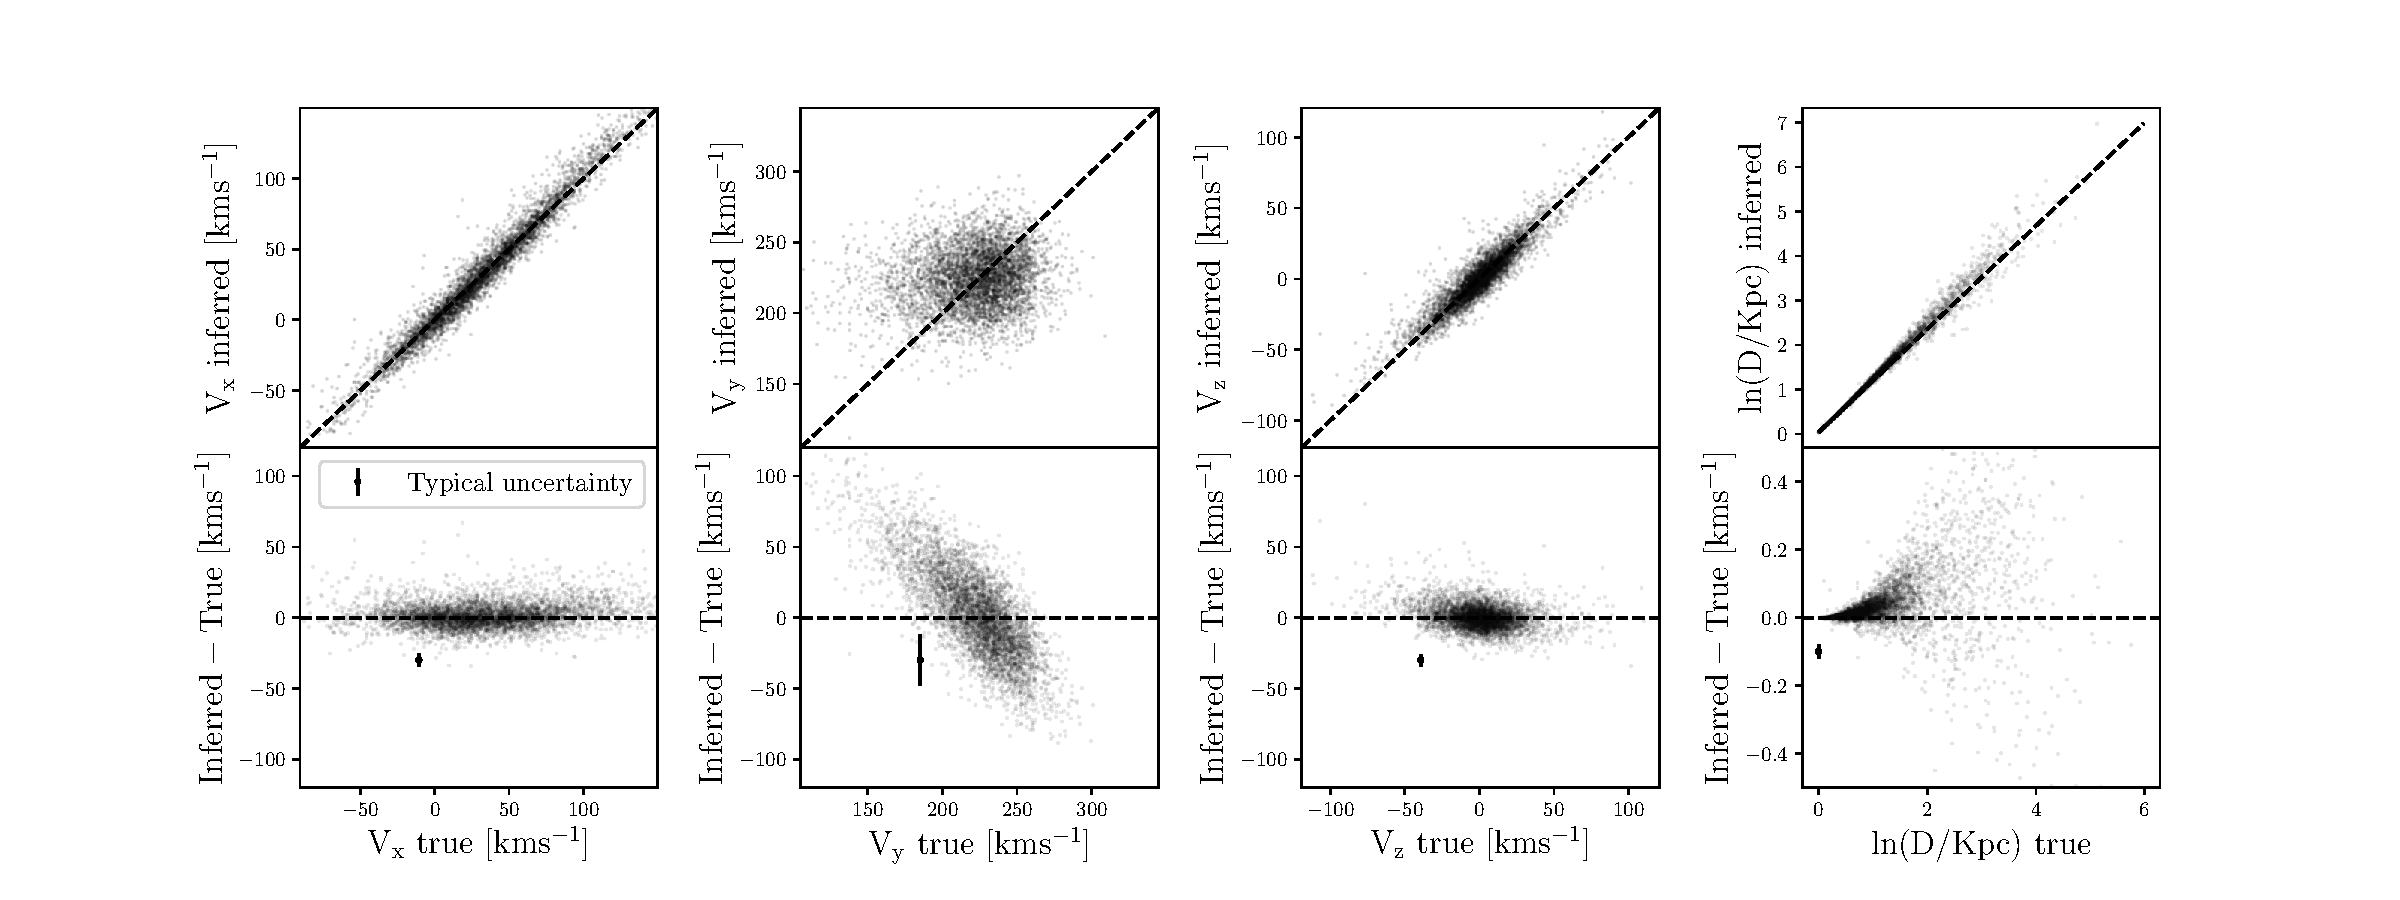
\includegraphics[width=1\textwidth]{residuals}
\label{fig:residuals}
\end{figure}
The three velocity components, \vx, \vy\ and \vz\ were recovered with
differing levels of precision: \vx\ and \vz\ are inferred more precisely than
\vy.
This is because of the position of the \kepler\ field, shown in figure
\ref{fig:kepler_field}.
The velocities of low-\vy\ stars are overestimated and the velocities of
high-\vy\ stars are underestimated.
This is because there is little information to constrain the \vy\ velocities
and the prior pulls the \vy\ velocities toward the center of the distribution.
The \vx, \vy\ and \vz\ velocities of stars are correlated, which means that
stars with an inaccurate \vy\ also have slightly accurate \vz\ and \vx.
Despite slight systematic inaccuracies visible in the residual (bottom)
panels of figure \ref{fig:residuals}, around 68\% of the inferred velocities
are within 1$\sigma$ of their true velocities; the inferred velocities are
consistent with the true velocities.

We provide a table of the directly-calculated, and indirectly-inferred 3D
velocities of stars observed by Kepler, in addition to their positional and
velocity information from Gaia EDR3, LAMOST DR5 and APOGEE DR16.
A description of each column included in that table is provided in table
\ref{tab:columns}.
% A sample of this table is displayed here, and the full machine-readable table
% is available online.

As briefly mentioned in the introduction, we have gone to the trouble of
inferring velocities in this paper because calculating velocities from proper
motions and distances alone, \ie\ assuming the RV is zero, will bias the
resulting velocities.
To demonstrate this, figure \ref{fig:inferred_vs_calc} shows the velocity
residuals for stars in our sample where we infer the velocities by
marginalizing over RV and where we ignore RV, \ie\ set it to zero.
In each panel, the green distributions show the residuals between the true
velocities and our inferred velocities, and the purple distributions show the
residuals between the true velocities and velocities calculated by setting the
RV to zero.
The median of each distribution is shown as a vertical line.
This figure shows that ignoring the RV dimension and assuming it can be set to
zero significantly biases the resulting velocities.
The correct way to de-bias velocity calculations is to marginalize over
missing RV measurements.
\begin{figure}[ht!]
\caption{
Residual velocity distributions calculated by marginalizing over missing RV
    measurements (green) or by assuming the RV can be set to zero (purple) for
    5000 stars in our sample.
Each distribution shows the residuals between the inferred/calculated
    velocities, and the velocities calculated using full 6D information:
    parallaxes, positions, proper motions, and RVs.
The vertical lines show the medians of each distribution.
This figure demonstrates that calculating stellar velocities using proper
    motions and distances alone will significantly bias the results.
Marginalizing over missing RV measurements ensures the resulting velocities
    will be unbiased.
}
  \centering
    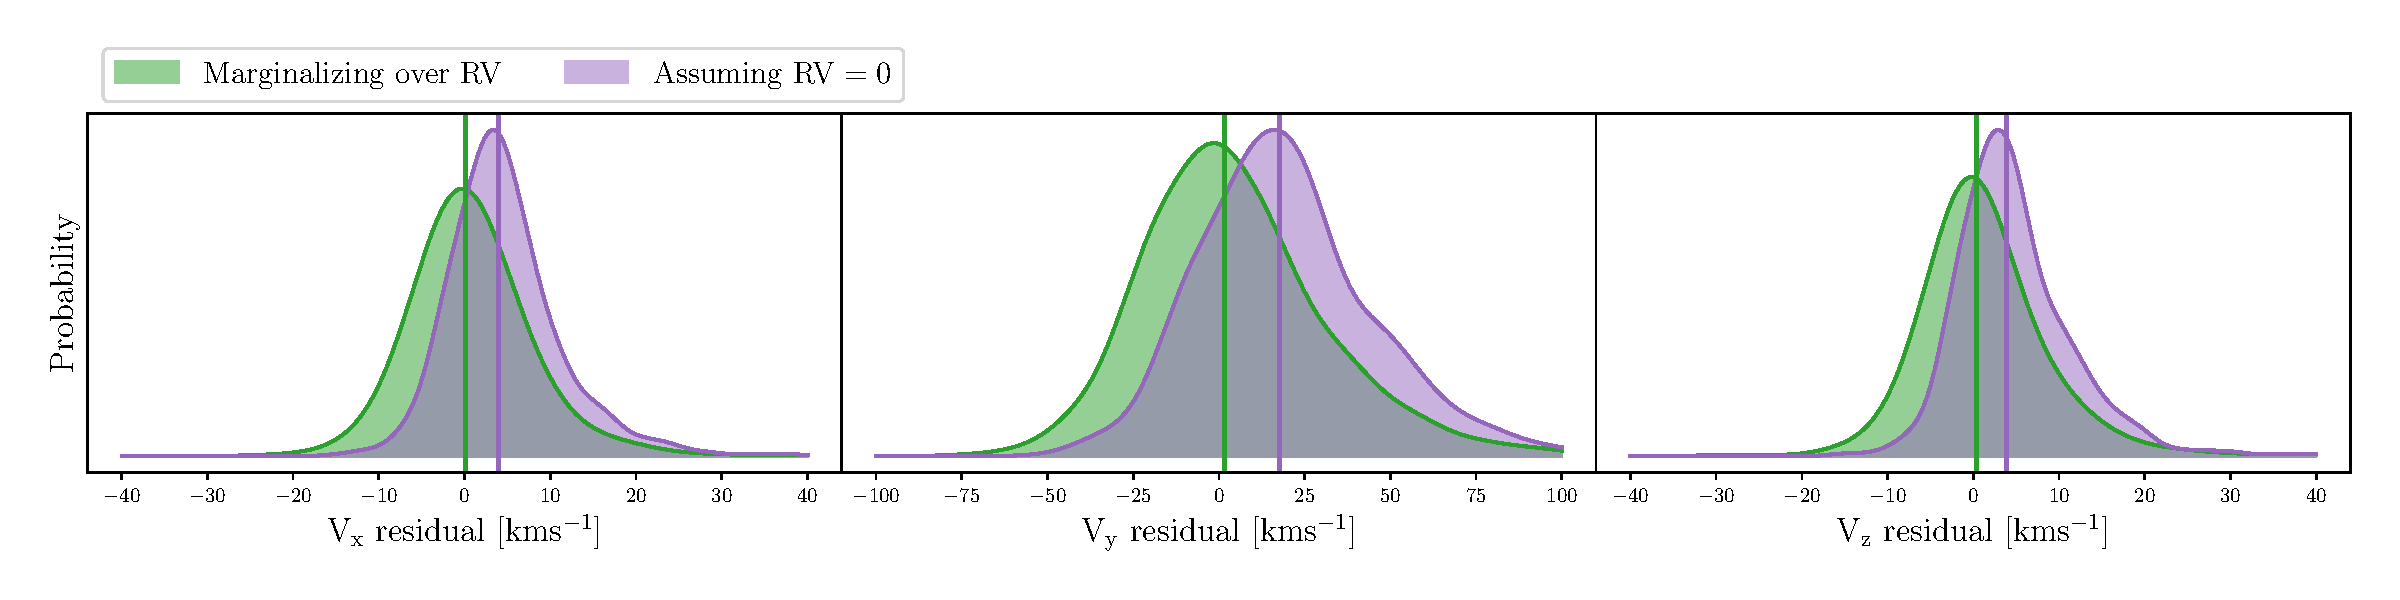
\includegraphics[width=1\textwidth]{inferred_vs_calc}
\label{fig:inferred_vs_calc}
\end{figure}

Our intention in providing a table of stellar velocities, and outlining our
method for inferring velocities without RV measurements, is to facilitate
kinematic age-dating studies.
The vertical velocities we provide could be used as an age proxy, or to
calculate kinematic ages via an age-velocity dispersion relation
\citep[\eg][]{yu2018, mackereth2019, sharma2021}.
This kind of approach has been used many times to examine the kinematic ages
of cool stars to explore stellar and planetary evolution
\citep[\eg][]{newton2016, kiman2019, hamer2019, angus2020, lu2021}.
For example, \citet{kiman2019} used the vertical velocity dispersions of stars
as an age proxy to explore the evolution of H$\alpha$ equivalent width (a
magnetic activity indicator), in M dwarfs.
\citet{hamer2019} compared the vertical velocity dispersions of stars with and
without hot Jupiters to show that hot Jupiter hosts tend to be younger, on
average, than stars without detected hot Jupiters.

% \begin{table}[h!]
%   \begin{center}
%       \caption{
% The velocities and kinematic information for the \nstars\ Kepler targets in
%       our sample.
%       The full list of columns is provided in table \ref{tab:columns} and the
%       full version is published in its entirey online.
%       }
% \label{tab:data}
% \begin{tabular}{cccccccccc}
%     KIC ID & DR3 source ID & $\alpha$ & $\delta$ & $\bar{\omega}$
%     & Distance & $\mu_{\alpha}$ & $\mu_\delta$ & RV (Gaia) & ... \\
%     & & $(^\circ)$ & $(^\circ)$ & mas & kpc & mas/yr & mas/yr & km/s & \\
%     {\tt kic$\_$id} & {\tt source$\_$id} & {\tt ra} & {\tt dec} &
%     {\tt parallax} & {\tt r$\_$est} & {\tt pmra} & {\tt pmdec} \\
% \hline
% ... & ... & ... & ... & ... & ... \\
% \end{tabular}
% \end{center}
% \tablecomments{This table is published in its entirety in a machine-readable format.
%       A portion is shown here for guidance regarding its form and content.}
% \ref{tab:data}
% \end{table}

\begin{table}[h!]
  \begin{center}
      \caption{
The list of columns in the data table published online, which provides
      the velocities and kinematic information for stars in the Kepler field.
      }
\label{tab:columns}
\begin{tabular}{cc}
    Column name & Description \\
\hline
    {\tt kic$\_$id} & The Kepler Input Catalog ID number of the target. \\
    {\tt source$\_$id} & The Gaia DR3 ID number of the target. \\
    {\tt ra, ra$\_$error} & Gaia EDR3 right ascenscion ($^\circ$). \\
    {\tt dec, dec$\_$error} & Gaia EDR3 declination in degrees ($^\circ$). \\
    {\tt parallax, parallax$\_$error} & Gaia EDR3 parallax (mas). \\
    {\tt r$\_$med$\_$photogeo, r$\_$lo$\_$photogeo, r$\_$hi$\_$photogeo} & Distance
    (parsec), provided by \citet{bailer-jones2021}. \\
    {\tt pmra, pmra$\_$error} & Gaia EDR3 proper motion in right ascension (mas/yr). \\
    {\tt pmdec, pmdec$\_$error} & Gaia EDR3 proper motion in declination (mas/yr). \\
    {\tt gaia$\_$dr2$\_$rv, gaia$\_$dr2$\_$rv$\_$error} & Gaia DR2 radial velocity (km/s) \\
    {\tt apogee$\_$rv, apogee$\_$rv$\_$error} & APOGEE DR16 radial velocity (km/s) \\
    {\tt lamost$\_$rv, lamost$\_$rv$\_$error} & LAMOST DR5 radial velocity (km/s) \\
    {\tt vx$\_$calc} & The \vx\ velocity calculated using RV (km/s). \\
    {\tt vx$\_$inferred, vx$\_$inferred$\_$error} & Median and std.
    dev, of \vx\ velocity samples, inferred without RV (km/s). \\
    {\tt vy$\_$calc} & The \vy\ velocity calculated using RV (km/s). \\
    {\tt vy$\_$inferred, vy$\_$inferred$\_$error} & Median and std.
    dev. of \vy\ velocity samples, inferred without RV (km/s). \\
    {\tt vz$\_$calc} & The \vz\ velocity calculated using RV (km/s). \\
    {\tt vz$\_$inferred, vz$\_$inferred$\_$error} & Median and std.
    devi. of \vz\ velocity samples, inferred without RV (km/s). \\
    {\tt vxvy$\_$covar} & The covariance between \vx\ and \vy\ samples. \\
    {\tt vxvz$\_$covar} & The covariance between \vx\ and \vz\ samples. \\
    {\tt vxlnd$\_$covar} & The covariance between \vx\ and $\ln$(distance)
    samples. \\
    {\tt vyvz$\_$covar} & The covariance between \vy\ and \vz\ samples. \\
    {\tt vylnd$\_$covar} & The covariance between \vy\ and $\ln$(distance)
    samples. \\
    {\tt vzlnd$\_$covar} & The covariance between \vz\ and $\ln$(distance)
    samples. \\
\end{tabular}
\end{center}
\end{table}
